\documentclass[tikz, border=10pt]{standalone}
\usepackage{iftex}
\ifluatex
  \usepackage{fontspec}
  \usepackage{unicode-math}
  \setmainfont{Fira Sans}
  \setmonofont{Fira Mono}
  \setmathfont{Fira Math}
\else
  \usepackage{newpxmath}
\fi

\usetikzlibrary{arrows.meta}
\tikzset{every node/.style={font=\Large}}


\begin{document}
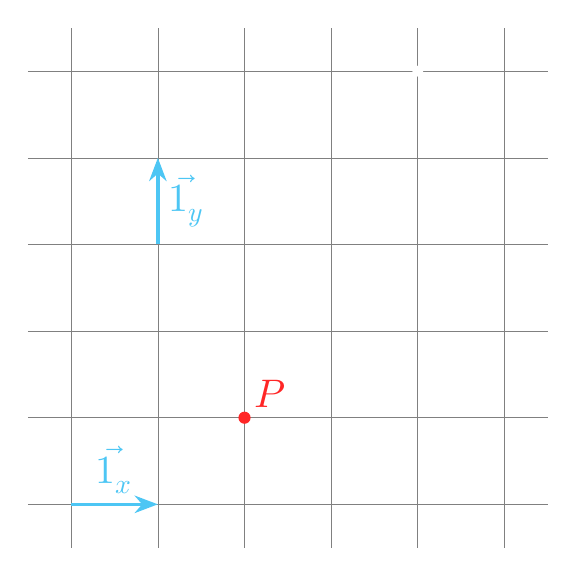
\begin{tikzpicture}[scale=1.1, >=Stealth]
  % Colors tuned for dark preview background.
  \colorlet{axiscol}{white}
  \colorlet{gridcol}{white!50!black}

  % Cartesian grid.
  \draw[step=1, very thin, gridcol] (-0.5,-0.5) grid (5.5,5.5);

  % Axes of the frame (O, i, j).
  % \draw[->, thick, axiscol] (-0.3,0) -- (5.6,0) node[below right, text=axiscol] {$x$};
  % \draw[->, thick, axiscol] (0,-0.3) -- (0,4.6) node[above left, text=axiscol] {$y$};

  % Basis vectors.
  \draw[->, very thick, cyan!70!white] (0,0) -- (1
  ,0)
    node[midway, above, text=cyan!70!white] {$\vec{1_x}$};
  \draw[->, very thick, cyan!70!white] (1,3) -- (1,4)
    node[midway, right, text=cyan!70!white] {$\vec{1_y}$};

  % Vector and its endpoint.
  \coordinate (P) at (2,1);
  \coordinate (O) at (4,5);
  
  % \draw[->, ultra thick, red!85!white] (A) -- (B);
    % node[midway, above left, text=red!85!white] {$\vec{u}$};

  % % Component projections.
  % \draw[dashed, thick, axiscol] (A) -- (4,0);
  % \draw[dashed, thick, axiscol] (A) -- (0,3);

  % Points and labels.
  \fill[axiscol] (O) circle (1.8pt);
  \fill[red!85!white] (P) circle (2pt);
  
  \node[below left, text=axiscol] at (O) {$O$};
  \node[above right, text=red!85!white] at (P) {$P$};
  
 
\end{tikzpicture}
\end{document}
